% -------------------------------------------------------------
% exercise_2.tex - Arknights Lone Trail pure TikZ vector asset
% Target: Replace 素材库/正文/exercise_2.png (252 x 161 bp)
% Supports dynamic colors: mibai, qiancheng, lv, huang, hong
% -------------------------------------------------------------
\ifcsname\string\color@mibai\endcsname\else\definecolor{mibai}{RGB}{244, 237, 218}\fi
\ifcsname\string\color@qiancheng\endcsname\else\definecolor{qiancheng}{RGB}{227, 101, 53}\fi
\ifcsname\string\color@lv\endcsname\else\definecolor{lv}{RGB}{131, 187, 170}\fi
\ifcsname\string\color@huang\endcsname\else\definecolor{huang}{RGB}{227, 164, 60}\fi
\ifcsname\string\color@hong\endcsname\else\definecolor{hong}{RGB}{149, 44, 38}\fi

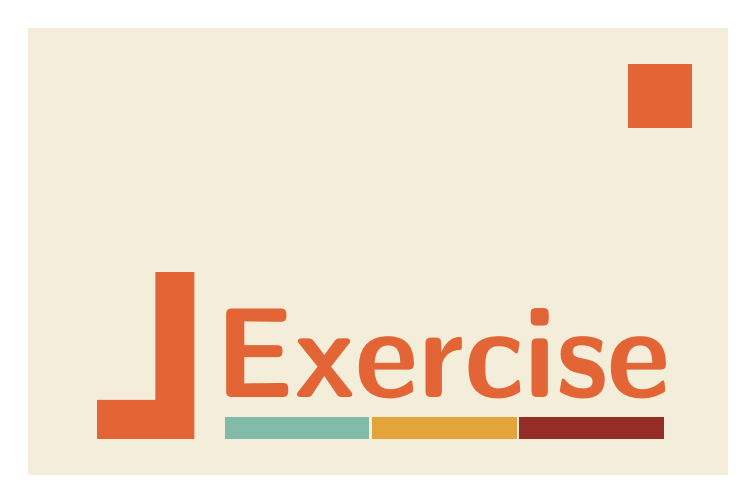
\begin{tikzpicture}[x=1bp, y=1bp, inner sep=0pt, outer sep=0pt]%
  % Bounding box & Background (exact 252 x 161 bp)
  \fill[mibai] (0, 0) rectangle (252, 161);

  % Upper-right orange square (23 x 23 bp, top margin 13 bp, right margin 13 bp)
  \fill[qiancheng] (216, 125) rectangle (239, 148);

  % Lower-left orange folded hook (base: 35 x 14 bp, stem: 14 x 46 bp)
  \fill[qiancheng] (25, 13) -- (60, 13) -- (60, 73) -- (46, 73) -- (46, 27) -- (25, 27) -- cycle;

  % Underline bars (height: 8 bp, Y: 13 to 21 bp)
  % Green bar (lv)
  \fill[lv] (71, 13) rectangle (123, 21);
  % Yellow bar (huang)
  \fill[huang] (124, 13) rectangle (176, 21);
  % Red bar (hong)
  \fill[hong] (177, 13) rectangle (229, 21);

  % Center text: Bold sans-serif "Exercise" (color: qiancheng)
  \node[anchor=south west, text=qiancheng, inner sep=0pt] at (67.5, 28) {%
    \resizebox{164bp}{32bp}{%
      \ifdefined\AvantGarde\AvantGarde\else\sffamily\bfseries\fi Exercise%
    }%
  };
\end{tikzpicture}%
